\documentclass[10pt,letterpaper]{article}
\usepackage[utf8]{inputenc}
\usepackage{amsmath}
\usepackage{amsfonts}
\usepackage{amssymb}

\usepackage[margin=0.5in]{geometry}		%used for margins
\usepackage{graphicx}					%used for images
\usepackage{booktabs}					%used for nicer tables
\pagenumbering{gobble}					%suppress page numbers

\title{Functional Testing - Decision Tables}
\author{
	Cai, Zelin\\
	\and
	Silvestre, Patrick\\
}
\date{}

\begin{document}
\maketitle
\newpage
\section{Workflow Diagram}
\begin{figure}[h]
	\centerline{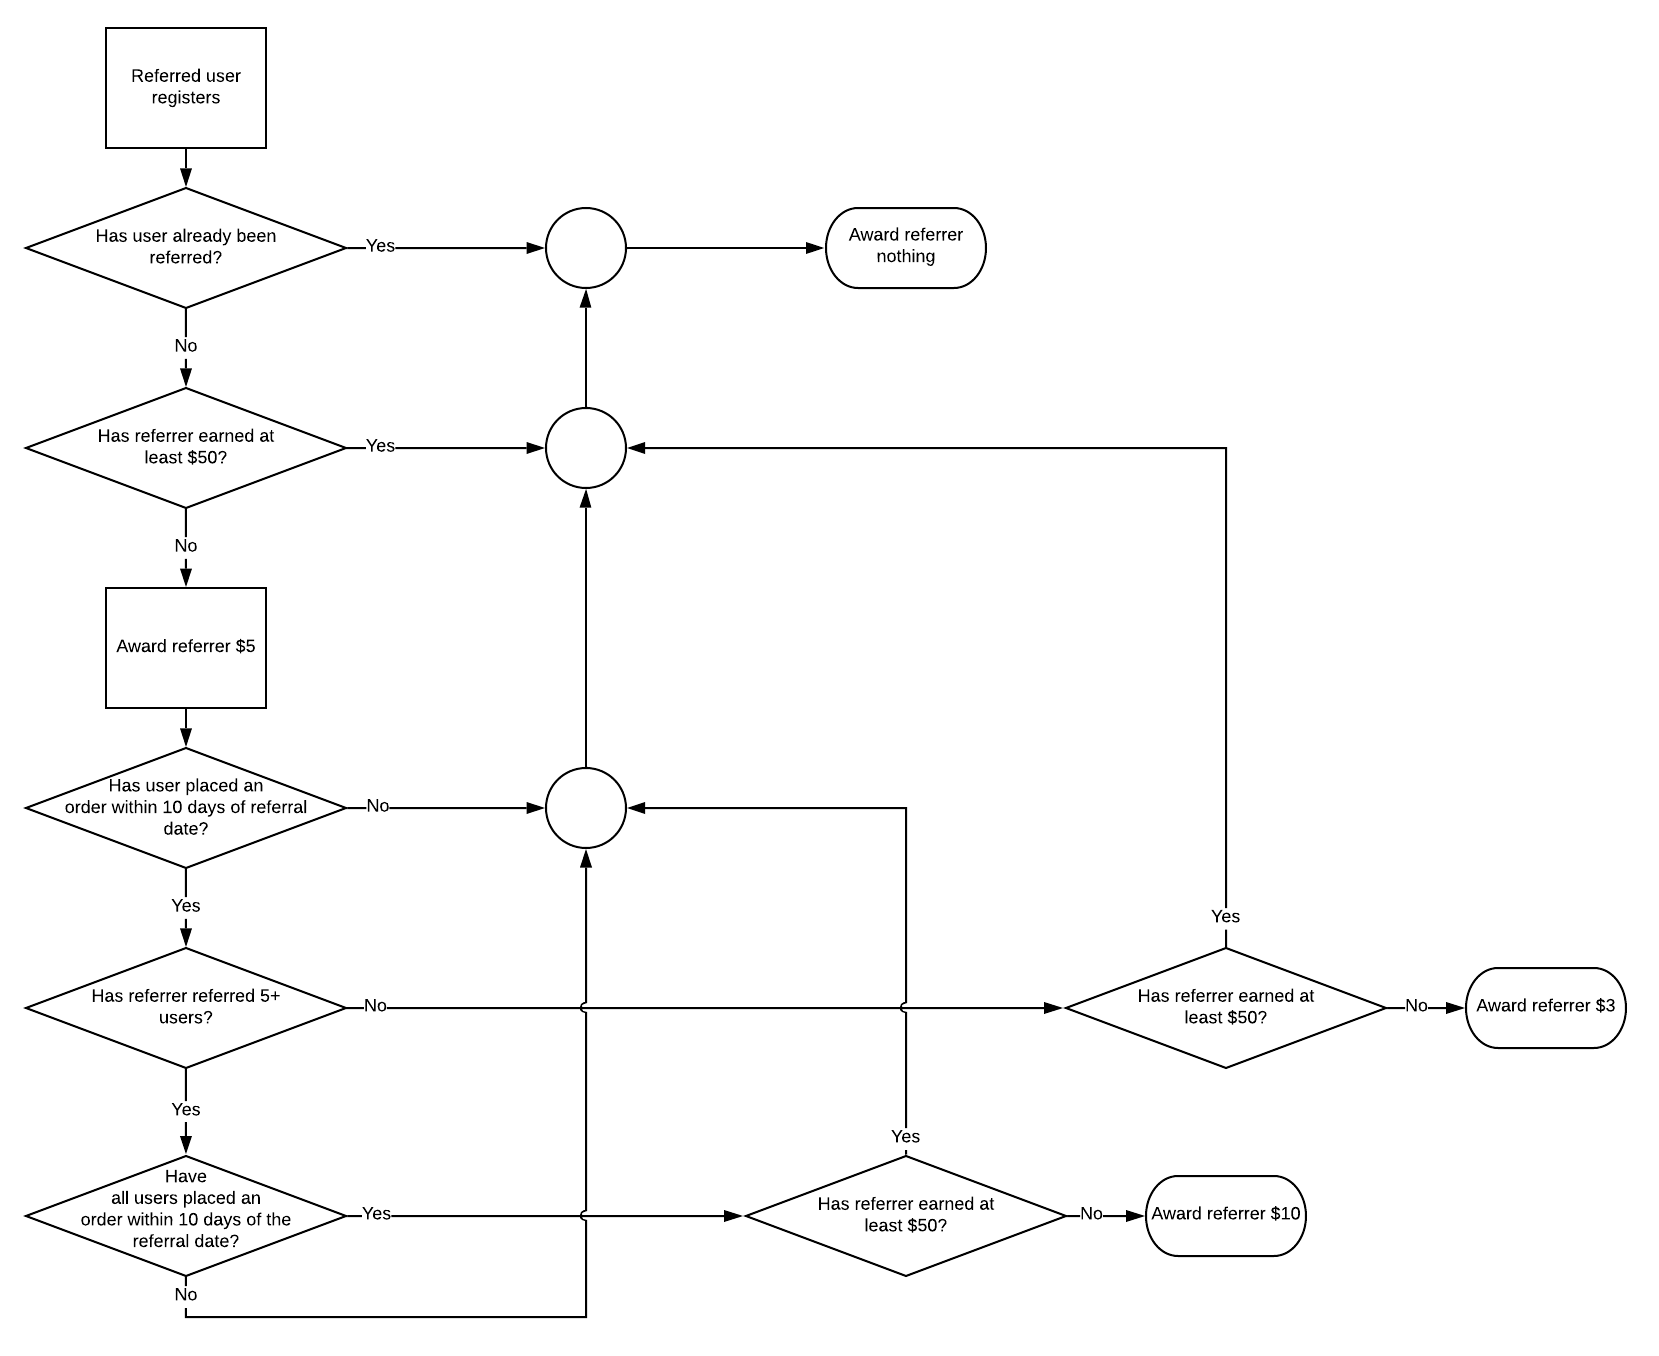
\includegraphics[width=9.5cm]{workflow.png}}
\end{figure}

\newpage
\section{Decision Table (Before Column Reduction)}
\begin{table}[h]
\begin{tabular}{@{}ll@{}}
\toprule
Condition & Explanation                                                                     \\ \midrule
$C_1$     & User is already referred                                                        \\ \midrule
$C_2$     & Referrer has earned more than \$50                                              \\ \midrule
$C_3$     & Referred user places an order within 10 days                                    \\ \midrule
$C_4$     & Referrer has referred 4+ additional users and all place an order within 10 days \\ \bottomrule
\end{tabular}
\end{table}

\begin{table}[h]
\begin{tabular}{@{}ll@{}}
\toprule
Effect & Explanation            \\ \midrule
$E_1$  & Award referrer nothing \\ \midrule
$E_2$  & Award referrer \$5     \\ \midrule
$E_3$  & Award referrer \$3     \\ \midrule
$E_4$  & Award referrer \$10    \\ \bottomrule
\end{tabular}
\end{table}

\begin{table}[h]
\begin{tabular}{@{}llllllllllllllllll@{}}
\toprule
                 &        & \multicolumn{16}{c}{Rules or Combinations}                           \\ \cmidrule(l){3-18} 
Conditions       & Values & 1 & 2 & 3 & 4 & 5 & 6 & 7 & 8 & 9 & 10 & 11 & 12 & 13 & 14 & 15 & 16 \\ \midrule
$C_1$            & Y, N   & Y & Y & Y & Y & Y & Y & Y & Y & N & N  & N  & N  & N  & N  & N  & N  \\
$C_2$            & Y, N   & Y & Y & Y & Y & N & N & N & N & Y & Y  & Y  & Y  & N  & N  & N  & N  \\
$C_3$            & Y, N   & Y & Y & N & N & Y & Y & N & N & Y & Y  & N  & N  & Y  & Y  & N  & N  \\
$C_4$            & Y, N   & Y & N & Y & N & Y & N & Y & N & Y & N  & Y  & N  & Y  & N  & Y  & N  \\
\textbf{Effects} &        &   &   &   &   &   &   &   &   &   &    &    &    &    &    &    &    \\
$E_1$            &        & 1 & 1 & 1 & 1 & 1 & 1 & 1 & 1 & 1 & 1  & 1  & 1  &    &    &    &    \\
$E_2$            &        &   &   &   &   &   &   &   &   &   &    &    &    & 1  & 1  & 1  & 1  \\
$E_3$            &        &   &   &   &   &   &   &   &   &   &    &    &    & 2  & 2  &    &    \\
$E_4$            &        &   &   &   &   &   &   &   &   &   &    &    &    & 3  &    &    &    \\ \bottomrule
\end{tabular}
\end{table}

\newpage
\section{Decision Table (After Column Reduction)}
\begin{table}[h]
\begin{tabular}{@{}ll@{}}
\toprule
Condition & Explanation                                                                     \\ \midrule
$C_1$     & User is already referred                                                        \\ \midrule
$C_2$     & Referrer has earned more than \$50                                              \\ \midrule
$C_3$     & Referred user places an order within 10 days                                    \\ \midrule
$C_4$     & Referrer has referred 4+ additional users and all place an order within 10 days \\ \bottomrule
\end{tabular}
\end{table}

\begin{table}[h]
\begin{tabular}{@{}ll@{}}
\toprule
Effect & Explanation            \\ \midrule
$E_1$  & Award referrer nothing \\ \midrule
$E_2$  & Award referrer \$5     \\ \midrule
$E_3$  & Award referrer \$3     \\ \midrule
$E_4$  & Award referrer \$10    \\ \bottomrule
\end{tabular}
\end{table}

\begin{table}[h]
\begin{tabular}{@{}lllllll@{}}
\toprule
                  &        & \multicolumn{5}{c}{Rules or Combinations} \\ \cmidrule(l){3-7} 
Conditions        & Values & 1      & 2      & 3      & 4      & 5     \\ \midrule
$C_1$             & Y, N   & Y      & N      & N      & N      & N     \\
$C_2$             & Y, N   & —      & Y      & N      & N      & N     \\
$C_3$             & Y, N   & —      & —      & Y      & Y      & N     \\
$C_4$             & Y, N   & —      & —      & Y      & N      & —     \\
\textbf{Effects}  &        &        &        &        &        &       \\
$E_1$             &        & 1      & 1      &        &        &       \\
$E_2$             &        &        &        & 1      & 1      & 1     \\
$E_3$             &        &        &        & 2      & 2      &       \\
$E_4$             &        &        &        & 3      &        &       \\ \midrule
\textbf{Checksum} & 16     & 8      & 4      & 1      & 1      & 2     \\ \bottomrule
\end{tabular}
\end{table}

\newpage
\section{Scenarios}
\subsection{Scenario 1}
Suppose:
\begin{itemize}
	\item{User is already referred}
	\item{Referrer has not earned at least \$50}
	\item{Referred user places an order within 10 days}
	\item{Referrer has not referred 4+ additional users}
\end{itemize}
Using the decision table, this scenario falls under rule 1. $C_1$ is true, and the remaining conditions do not have an impact on the final effect: $E_1$.

\subsection{Scenario 2}
Suppose:
\begin{itemize}
	\item{User is not already referred}
	\item{Referrer has earned at least \$50}
	\item{Referred user places an order within 10 days}
	\item{Referrer has not referred 4+ additional users}
\end{itemize}
Using the decision table, this scenario falls under rule 2. $C_1$ is false, $C_2$ is true, and the remaining conditions do not have an impact on the final effect: $E_1$.

\subsection{Scenario 3}
Suppose:
\begin{itemize}
	\item{User is not already referred}
	\item{Referrer has not earned at least \$50}
	\item{Referred user does not place an order within 10 days}
	\item{Referrer has not referred 4+ additional users}
\end{itemize}
Using the decision table, this scenario falls under rule 5. $C_1$, $C_2$, and $C_3$ are false, and the remaining condition does not have an impact on the final effect: $E_2$.

\end{document}